\if0
☆レポート課題(チームで一部だけ提出して下さい)

1. 表紙(課題名、チームメンバ氏名、提出日)

2. SingleCycleMIPSのモジュール仕様書
 設計した各モジュールについて、上位階層から順に、下記の内容をまとめること。
 ・モジュール名
 ・モジュールの入出力信号名とその説明

例: 入力信号一覧
name 	width 	explanation
CLK 	[0:0] 	SingleCycleMIPS用クロック信号
PC 	[31:0] 	次に実行する命令アドレスを格納するレジスタ値


 ・モジュール内のブロック図(サブモジュール間の接続関係を明示すること。ただし、最下層のIF, ID, EX, MAについては、ブロック図は不要です。)
 ・モジュールの動作の説明文

3. 実機DE10-Liteでの動作検証
 ・テストプログラムのファイル名一覧(load_store, arithmetic, array, if_then_else, while, function, recursion, hanoi)
 ・テストプログラムの実行方法
 ・テストプログラムの検証法
 ・各テストプログラムの検証結果

4. 考察(メンバ一人づつ、個別の考察を記述して下さい。1600文字以上/人)
 ・今回の回路設計で工夫した点(技術的な視点、チーム内での役割分担等のプロジェクト管理的な視点)
 ・より実用的なMIPSプロセッサを実現するために、マイクロアーキテクチャの観点から改良すべき点、および、それに関連して追加で実装すべき機能/回路

5. 感想(メンバ一人づつ、個別の感想を記述して下さい。800文字程度)

6.参考文献
\fi
\documentclass[dvipdfmx]{jsarticle}
\usepackage{graphicx}[dvipdfmx]
\usepackage{multirow}
\usepackage{array}
\usepackage{amsmath,amssymb}
\usepackage{url}
\usepackage{listings}
\usepackage{color}
\usepackage{verbatim}

\title{計算機設計論 レポート課題:MIPSプロセッサの回路設計}
\author{1295149 森岡悠人\\}
\date{\today}

\begin{document}
\maketitle

\section{モジュール仕様書}


QuartusのRTL Viewerを用いて出力した,DE10-liteに書き込んだモジュールのブロック図を図\ref{fig:rtl}に示す.
\begin{figure}[h]
\centering
  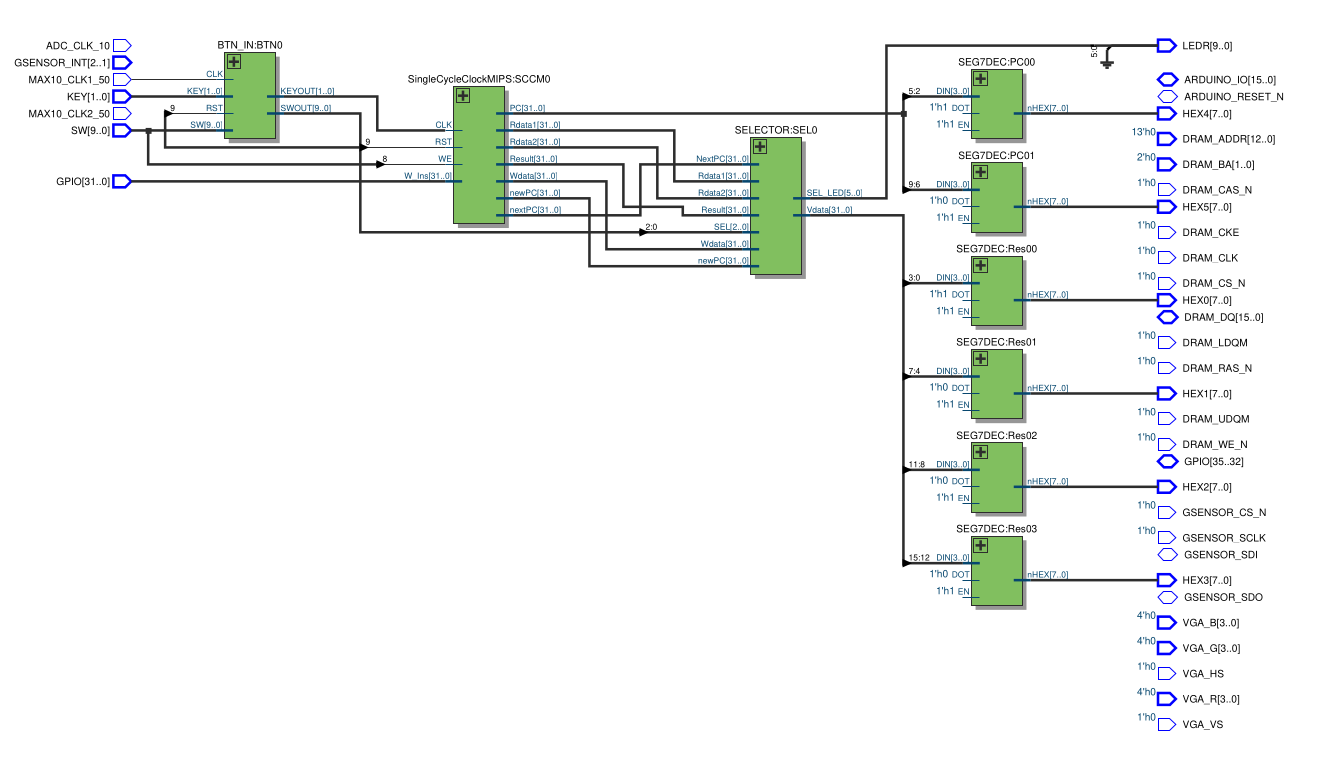
\includegraphics[width=\textwidth]{myRTL.png}
  \caption{作成したMIPS回路のブロック図}
  \label{fig:rtl}
\end{figure}



\section{動作検証}
作成したverilogコードがMIPSの命令セットを実行できるかどうかの検証を行った.
テストプログラムとして,教科書\cite{textbook}に掲載されているアセンブラプログラム(load\_store, arithmetic, array, if\_then\_else, while, function, recursion, hanoi)を用いた.
プログラムはCPUlator MIPS System Simulator \cite{mips-sim}を用いてコンパイルした.
その後32bitの16進数で出力されたバイナリを\texttt{IMem.txt}に書き込んでおき,IMに読み込ませた状態でシミュレーションを実行した.
動作の流れとデータメモリの中身を確認するため,modelsim20.1を用いて動作のシミュレーションと検証を行った.
シミュレーション結果は,display命令を用いて,PC, Instruction, ALU\_resultレジスタの順番が期待通りかどうかを確認した.
シミュレーションの様子を図\ref{fig:simulation}に示す.
\begin{figure}[h]
\centering
  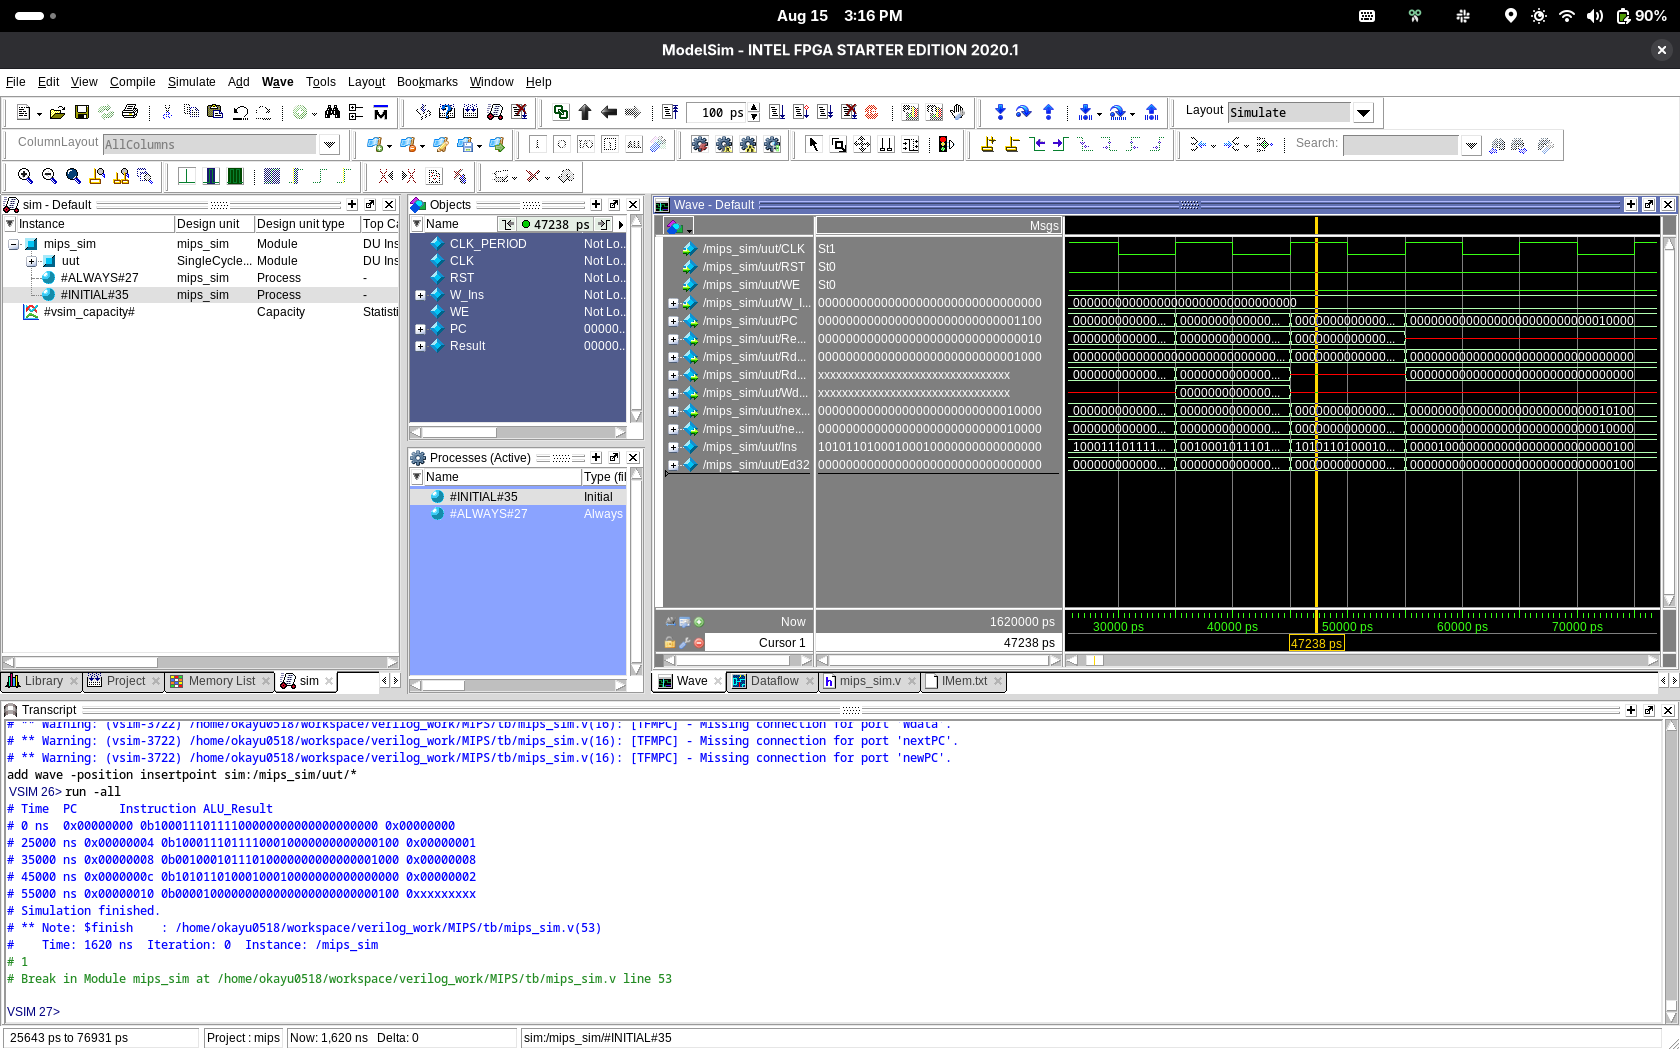
\includegraphics[width=0.8\textwidth]{modelsim.png}
  \caption{modelsimによるシミュレーションの様子}
  \label{fig:simulation}
\end{figure}

\subsection{test: load\_store}
基本的なロードストア命令の動作確認を行った.使用したアセンブリコードは付録\ref{appendix:load_store_asm}に示す.詳細なテスト結果は付録\ref{appendix:load_store}に示す.

\subsection{test: arithmetic}
あらかじめテストベンチでDMemの0番地からそれぞれ変数a=1,b=2,c=3,d=0と変数のオフセットを保持するレジスタ\$s7=0を初期値として設定してシミュレーションを実行した.
その結果,期待通りa, b, cの値がadd命令で足し合わされ,\$s3=6であることを確認した.使用したアセンブリコードは付録\ref{appendix:arithmetic_asm}に示す.詳細なテスト結果は付録\ref{appendix:arithmetic}に示す.

\subsection{test: array}
あらかじめテストベンチでDMemの0番地からそれぞれ配列a[0]=0, a[1]=1..., a[9]=9と配列のオフセットを保持するレジスタ\$s7=0と\$s2=2を初期値として設定してシミュレーションを実行した.
その結果,期待通り\$s1=2, \$s2=5であることを確認した.使用したアセンブリコードは付録\ref{appendix:array_asm}に示す.詳細なテスト結果は付録\ref{appendix:array}に示す.

\subsection{test: if\_then\_else}
まず,if文が真になる場合のテストを行った.
あらかじめテストベンチでレジスタ\$s0=0xa, \$s1=0xa, \$s2=0x0を初期値として設定してシミュレーションを実行した.
その結果,\$s0と\$s1が等しいため,\$s2に\$s1の値が代入され,\$s2=0xaであることを確認した.
次に,if文が偽になる場合のテストを行った.
あらかじめテストベンチでレジスタ\$s0=0xa, \$s1=0xb, \$s2=0x0を初期値として設定してシミュレーションを実行した.
その結果,\$s0と\$s1が等しくないため,\$s2に\$s0の値が代入され,\$s2=0xaであることを確認した.
真の場合と偽の場合のPCの遷移を比べると,偽の場合はelse節のラベルを飛び越えるためにJ命令が実行されているためことがわかる.
そのため偽の場合は1命令多い.使用したアセンブリコードは付録\ref{appendix:if_then_else_asm}に示す.詳細なテスト結果は付録\ref{appendix:if_then_else}に示す.

\subsection{test: while}
あらかじめテストベンチで配列a[10]を0で初期化し,配列のオフセットを保持するレジスタ\$s7=0, \$s0=0を初期値として設定してシミュレーションを実行した.
その結果,\$s0が10になるまでwhile文が繰り返され,配列a[0]からa[9]にそれぞれ0から9までの値が代入されていることを確認した.使用したアセンブリコードは付録\ref{appendix:while_asm}に示す.詳細なテスト結果は付録\ref{appendix:while}に示す.

\subsection{test: function}
\label{sec:function}
あらかじめテストベンチでレジスタ\$s0=10を初期値として設定して1からnまでの和を求めるプログラムのシミュレーションを実行した.
その結果,\$s1=0x37=0d55となることを確認した.使用したアセンブリコードは付録\ref{appendix:function_asm}に示す.詳細なテスト結果は付録\ref{appendix:function}に示す.

\subsection{test: recursion}
\ref{sec:function}のテストと同様に,あらかじめテストベンチでレジスタ\$s0=10を初期値として設定してシミュレーションを実行した.
その結果,\$s1=0x37=0d55となることを確認した.使用したアセンブリコードは付録\ref{appendix:recursion_asm}に示す.詳細なテスト結果は付録\ref{appendix:recursion}に示す.

\subsection{test: hanoi}
円盤が3枚のハノイの塔を解くプログラムを実行する.
レジスタ\$t1を移動回数カウント用としてシミュレーションを行った.
結果,\$t1=7となり,期待通りの動作を確認した.
hanoiのテストは算術演算,関数呼び出しなど,上記の多くの処理を含むため,Quartus Primeを用いてDE10-Liteに書き込んで実行した.
その結果,modelsim同様に期待通りの動作をし,最後の無限ループの処理まで到達することを確認できた.使用したアセンブリコードは付録\ref{appendix:hanoi_asm}に示す.詳細なテスト結果は付録\ref{appendix:hanoi}に示す.



\section{考察}



\section{感想}



\appendix
\section{テストプログラム}

本節では、各テストプログラムのアセンブリコードとその動作について説明する。

\subsection{load\_storeプログラム}
\label{appendix:load_store_asm}
このプログラムは基本的なロード・ストア命令の動作を確認するためのテストである。
プログラムでは、データメモリから値をロードし、別のアドレスにストアする処理を行う。
\verbatiminput{test-results/load_store.asm}

\textbf{プログラムの動作:}
\begin{itemize}
\item \texttt{lw \$s0, 0(\$s7)}: データメモリのアドレス\texttt{\$s7+0}から値をロードし、\texttt{\$s0}に格納
\item \texttt{lw \$s1, 4(\$s7)}: データメモリのアドレス\texttt{\$s7+4}から値をロードし、\texttt{\$s1}に格納  
\item \texttt{addi \$t0, \$s7, 8}: \texttt{\$s7+8}をアドレスとして\texttt{\$t0}に計算
\item \texttt{sw \$s1, 0(\$t0)}: \texttt{\$s1}の値を\texttt{\$t0}が示すアドレスにストア
\end{itemize}

\subsection{arithmeticプログラム}
\label{appendix:arithmetic_asm}
このプログラムは基本的な算術演算命令の動作を確認するためのテストである。
3つの値を読み込んで加算を行い、結果をレジスタに格納する。

\verbatiminput{test-results/arithmetic.asm}

\textbf{プログラムの動作:}
\begin{itemize}
\item 変数a, b, cの値(1, 2, 3)をそれぞれ\texttt{\$s0}, \texttt{\$s1}, \texttt{\$s2}にロード
\item \texttt{add \$t0, \$s0, \$s1}: a + b の結果を\texttt{\$t0}に格納
\item \texttt{add \$s3, \$t0, \$s2}: (a + b) + c の結果を\texttt{\$s3}に格納(期待値:6)
\end{itemize}

\subsection{arrayプログラム}
\label{appendix:array_asm}
このプログラムは配列のアクセスとインデックス計算の動作を確認するためのテストである。

\verbatiminput{test-results/array.asm}

\textbf{プログラムの動作:}
\begin{itemize}
\item \texttt{sll \$t0, \$s0, 2}: インデックス\texttt{\$s0}を4倍(左シフト2ビット)してワードアドレスに変換
\item \texttt{add \$t0, \$s7, \$t0}: 配列の基底アドレス\texttt{\$s7}にオフセットを加算
\item \texttt{lw \$s1, 0(\$t0)}: 計算されたアドレスから配列要素をロード
\item \texttt{lw \$s2, 20(\$s7)}: 配列の5番目の要素(20バイトオフセット)をロード
\end{itemize}

\subsection{if\_then\_elseプログラム}
\label{appendix:if_then_else_asm}
このプログラムは条件分岐命令の動作を確認するためのテストである。

\verbatiminput{test-results/if_then_else.asm}

\textbf{プログラムの動作:}
\begin{itemize}
\item \texttt{beq \$s0, \$s1, L1}: \texttt{\$s0}と\texttt{\$s1}が等しい場合はL1にジャンプ
\item 等しくない場合:\texttt{\$s2 = \$s0}を実行してN1にジャンプ
\item 等しい場合(L1):\texttt{\$s2 = \$s1}を実行
\end{itemize}

\subsection{whileプログラム}
\label{appendix:while_asm}
このプログラムはループ処理と条件判定の動作を確認するためのテストである。

\verbatiminput{test-results/while.asm}

\textbf{プログラムの動作:}
\begin{itemize}
\item \texttt{slti \$t0, \$s0, 10}: \texttt{\$s0 < 10}の条件判定結果を\texttt{\$t0}に格納
\item 条件が偽(\texttt{\$s0 >= 10})の場合はループを終了してN1にジャンプ
\item 条件が真の場合:配列に\texttt{\$s0}の値を格納し、\texttt{\$s0}をインクリメントしてループを継続
\end{itemize}

\subsection{functionプログラム}
\label{appendix:function_asm}
このプログラムは関数呼び出しとスタック操作の動作を確認するためのテストである。
1からnまでの和を計算する関数を実装している。

\verbatiminput{test-results/function.asm}

\textbf{プログラムの動作:}
\begin{itemize}
\item メイン部分:引数を\texttt{\$a0}に設定してsum関数を呼び出し、戻り値を\texttt{\$s1}に格納
\item sum関数:スタックにレジスタを退避し、1からnまでの和を計算して\texttt{\$v0}に結果を返す
\item 関数終了時にはスタックからレジスタを復元し、呼び出し元に戻る
\end{itemize}

\subsection{recursionプログラム}
\label{appendix:recursion_asm}
このプログラムは再帰関数呼び出しの動作を確認するためのテストである。
再帰を用いて1からnまでの和を計算する。

\verbatiminput{test-results/recursion.asm}

\textbf{プログラムの動作:}
\begin{itemize}
\item 引数が1未満の場合は0を返してベースケースとする
\item 引数が1以上の場合は、引数を1減らして再帰呼び出しを行い、その結果に現在の引数値を加算
\item 各再帰レベルでスタックに引数と戻りアドレスを保存・復元
\end{itemize}

\subsection{hanoiプログラム}
\label{appendix:hanoi_asm}
このプログラムはハノイの塔を解く再帰アルゴリズムを実装し、複雑な再帰処理の動作を確認するためのテストである。

\verbatiminput{test-results/hanoi.asm}

\textbf{プログラムの動作:}
\begin{itemize}
\item 3枚の円盤のハノイの塔問題を解く
\item \texttt{\$a0}: 円盤の枚数、\texttt{\$a1}: 移動元、\texttt{\$a2}: 移動先、\texttt{\$a3}: 補助杆
\item \texttt{\$t1}: 移動回数カウンタ(期待値:7回)
\item 再帰の深さに応じてスタックに多くの引数と戻りアドレスを保存
\item ベースケース(円盤が1枚)では直接移動を実行
\end{itemize}

\section{テスト結果詳細}

\subsection{load\_storeのテスト結果}
\label{appendix:load_store}
\verbatiminput{test-results/load_store.txt}

\subsection{arithmeticのテスト結果}
\label{appendix:arithmetic}
\verbatiminput{test-results/arithmetic.txt}

\subsection{arrayのテスト結果}
\label{appendix:array}
\verbatiminput{test-results/array.txt}

\subsection{if\_then\_elseのテスト結果(真の場合)}
\label{appendix:if_then_else}
\verbatiminput{test-results/if_then_else_true.txt}

\subsubsection{if\_then\_elseのテスト結果(偽の場合)}
\verbatiminput{test-results/if_then_else_false.txt}

\subsection{whileのテスト結果}
\label{appendix:while}
\verbatiminput{test-results/while.txt}

\subsection{functionのテスト結果}
\label{appendix:function}
\verbatiminput{test-results/function.txt}

\subsection{recursionのテスト結果}
\label{appendix:recursion}
\verbatiminput{test-results/recursion.txt}

\subsection{hanoiのテスト結果}
\label{appendix:hanoi}
\verbatiminput{test-results/hanoi.txt}


\bibliographystyle{junsrt}
\bibliography{refs}
\end{document}

